%==============================================================================
%== template for LATEX poster =================================================
%==============================================================================
%
%--A0 beamer slide-------------------------------------------------------------
\documentclass[final]{beamer} % use beamer
\usepackage[orientation=portrait,
            size=a1,          % poster size
            scale=0.714        % font scale factor
           ]{beamerposter}    % beamer in poster size
%
%--some needed packages--------------------------------------------------------
\usepackage[american]{babel}  % language 
\usepackage[utf8]{inputenc}   % std linux encoding
%
%==The poster style============================================================
\usetheme{cpbgposter}            % our poster style
%--set colors for blocks (without frame)---------------------------------------
  \setbeamercolor{block title}{fg=ngreen,bg=white}
  \setbeamercolor{block body}{fg=black,bg=white}
%--set colors for alerted blocks (with frame)----------------------------------
%--textcolor = fg, backgroundcolor = bg, dblue is the jacobs blue
  \setbeamercolor{block alerted title}{fg=white,bg=hblue}%frame color
  \setbeamercolor{block alerted body}{fg=black,bg=hblue!10}%body color
%
%==Titel, date and authors of the poster=======================================
\title{Top background to Supersymmetry searches in dilepton events}
\author{Timothy Brooks (brooks@cern.ch)}
\institute{Royal Holloway, University of London}
\date{\today}
%
%==some usefull qm commands====================================================
%  |x>
\newcommand{\ket}[1]{\left\vert#1\right\rangle}
%  <x|
\newcommand{\bra}[1]{\left\langle#1\right\vert}
%  <x|y>
\newcommand{\braket}[2]{\left< #1 \vphantom{#2}\,
                        \right\vert\left.\!\vphantom{#1} #2 \right>}
%  <x|a|y>
\newcommand{\sandwich}[3]{\left< #1 \vphantom{#2 #3} \right|
                          #2 \left|\vphantom{#1 #2} #3 \right>}
%  d/dt
\newcommand{\ddt}{\frac{d}{dt}}
%  D/Dx
\newcommand{\pdd}[1]{\frac{\partial}{\partial#1}}
%  |x|
\newcommand{\abs}[1]{\left\vert#1\right\vert}
%  k_{x}
\newcommand{\kv}[1]{\mathbf{k}_{#1}}
%==============================================================================
%==the poster content==========================================================
%==============================================================================
\begin{document}
%--the poster is one beamer frame, so we have to start with:
\begin{frame}[t]
%--to seperate the poster in columns we can use the columns environment
 \begin{columns}[t] % the [t] options aligns the columns content at the top
%--the left column-------------------------------------------------------------
  \begin{column}{0.28\paperwidth}% the right size for a 3-column layout
%--abstract block--------------------------------------------------------------
   \begin{alertblock}{Abstract}
    Searches for Supersymmetry with two lepton final states are limited by
    backgrounds from events with top quark pairs. Top events mimic many of
    the characteristics of events involving supersymmetric particles including
    leptons, jets and missing energy. The discovery significance of a search,
    then, must account for the top contribution. In
    addition, uncertainty in the size of this contribution degrades the
    significance of a search. Presented here is a method to measure the top
    background from data with a smaller uncertainty than estimates from Monte
    Carlo simulations.
   \end{alertblock}
   \vskip2ex
%--Remarks block----------------------------------------------------------------
   \begin{block}{Selection variables}
    In searching for events characteristic of Supersymmetry, variables that
    strongly descriminate against standard model proccesses are defined. The
    event variables used in this analysis are as follows:
    \begin{itemize}
      \item Missing transverse energy, $E_{T}^{miss} \equiv \left|
      \displaystyle\sum\limits_{i}^{N}-\vec{E}_{T,i} \right|$
      \vskip1ex
      \item Effective mass, $M_{eff} \equiv \displaystyle\sum\limits_{i=1}^{4}
      P_{T}^{jet, i} + \displaystyle\sum\limits_{i=1} P_{T}^{lep, i} +
      E_{T}^{miss}$
      \vskip1ex
      \item Transverse sphericity, $S_{T} \equiv \frac{2 \lambda_{2}}{\left(
      \lambda_{1} + \lambda_{2} \right)}$ where $\lambda_{1}$ \& $\lambda_{2}$
      are eigenvalues of the sphericity tensor (see Ref.\cite{CSCSUSY}).
    \end{itemize}
    \vskip1ex
    Events involving supersymmetric particles are expected to yeild high
    effective masses, significant missing energy and have uniform sphericities
    up to 1. In addition to these variables, multiplicities and transverse
    momenta $\left(P^{T}\right)$ for individual particles detected in events
    are part of selection. Below is a selection criteria for events with two
    leptons.
   \end{block}
   \vskip1ex
%--features block---------------------------------------------------------------
   \begin{block}{Sample selection}
    Fig.~\ref{fig:susydoubledecay} is an example final state that this search
    would be sensitive to. The final state leaves 2 leptons, 2 light quarks and
    missing energy in the form of neutrinos and the lightest supersymmetric
    particle (LSP), in this model, the neutralino. Reference \cite{7tevNote}
    demonstrates searches for events including 0, 1 and 2 leptons in the final
    state. The search in this analysis, with 2 oppositely signed leptons, is
    further broken down into 3 selections for events with at least 2, 3 or 4
    jets. These selections are defined as follows:
    \begin{enumerate}
      \item Exactly two leptons with $P_{T} > 10$~GeV and opposite charge.
      \item $\geq [2,3,4]$ jets with $P_{T} > [50,40,40]$~GeV and a leading jet
      $P_{T} > [180,100,100]$~GeV
      \item Missing transverse energy $E_{T}^{miss} > 80$~GeV.
      \item $\Delta\phi( jet_{i},E_{T}^{miss} ) > 0.2$ for the $[2,3,3]$ leading
      jets.
      \item $E_{T}^{miss} > [0.3,0.25,0.2] \times M_{eff}$.
      \item Transverse sphericity, $S_{T} > 0.2$.
    \end{enumerate}
    The distribution of transverse sphericity before the last cut is shown in
    Fig.~\ref{fig:Canvas2j} and Fig.~\ref{fig:Canvas4j}. This shows the higher
    purity in the selected region to the right. Using these cuts, we can predict
    the expected number of signal and background events from Monte Carlo.
   \end{block}
   \vskip1ex
   
   \begin{block}{Monte Carlo results}
    Table \ref{tb:results} shows signal and background expectation values
    from Monte Carlo analysis normalised to one inverse femtobarn. These
    values are consistent with the findings of \cite{7tevNote}. Samples analysed
    at $7$~TeV with full GEANT4 ATLAS detector simulation and reconstruction:
      \begin{itemize}
        \item SUSY benchmark point 4 (JIMMY) 50,000 events.
        \item $t\bar{t}$ produced with (POWHEG + PYTHIA) 200,000 events.
        \item $WZ$ + jets produced with (ALPGEN + JIMMY) 35,000 events.
      \end{itemize}
      \begin{table}
       \begin{tabular}{|r|c | c | c|}\hline
        & 2jet & 3jet & 4jet \\
        \hline
        Signal (SU4) & 38.82 & 112.74 & 90.76 \\
        Background ($t\bar{t}$) & 3.48 & 37.89 & 20.90 \\
        \hline
        \multicolumn{4}{|c|}{ATLAS work in progress} \\
        \hline
       \end{tabular}
       \caption{Signal and background values for 2, 3 \& 4 jet analyses.}
       \label{tb:results}
      \end{table}
   \end{block}
  \end{column}


  \begin{column}{0.60\paperwidth}
    \begin{figure}\centering
     \begin{minipage}[c]{.45\textwidth}\centering
      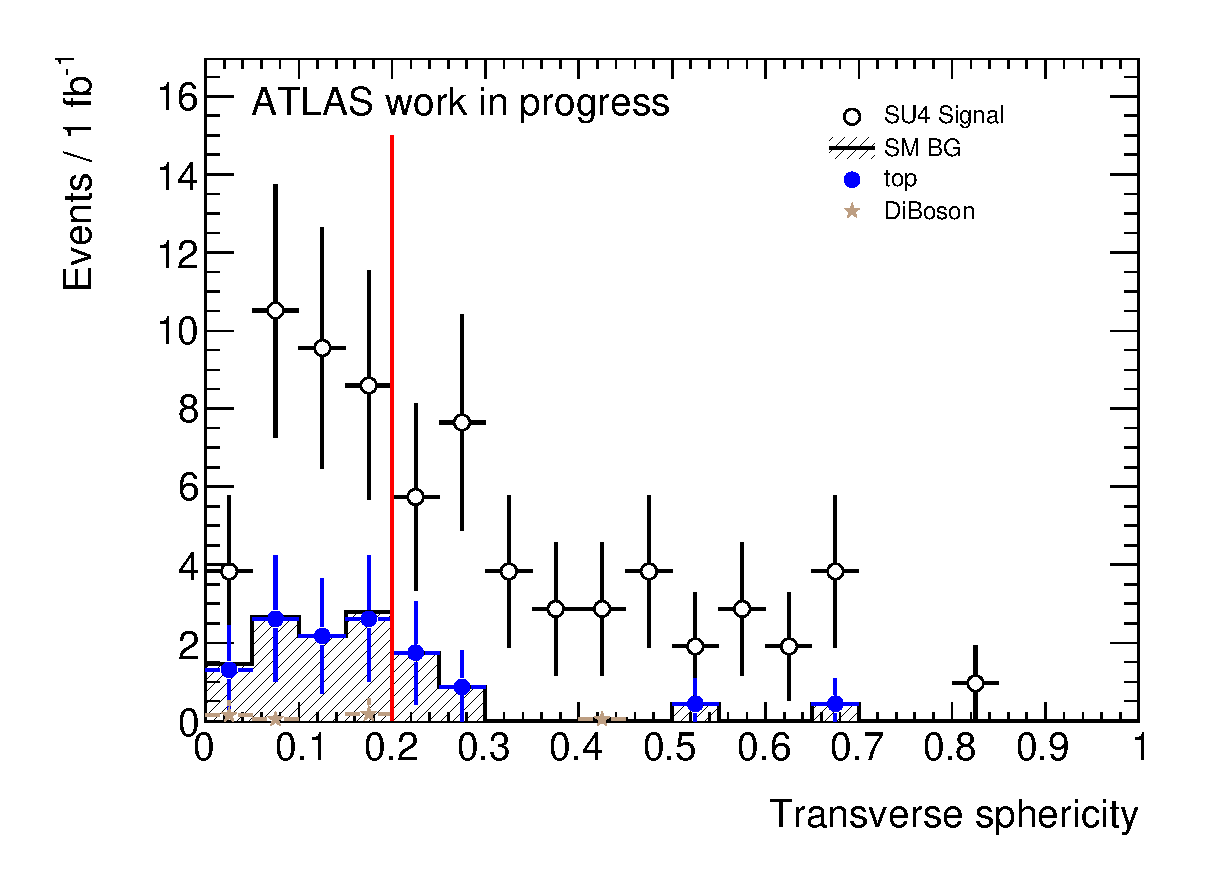
\includegraphics[width=.9\textwidth]{img/Canvas2j}
      \caption{Transverse sphericity distribution after 2 jet selection.}
      \label{fig:Canvas2j}
     \end{minipage}\hfill
     \begin{minipage}[c]{.45\textwidth}\centering
      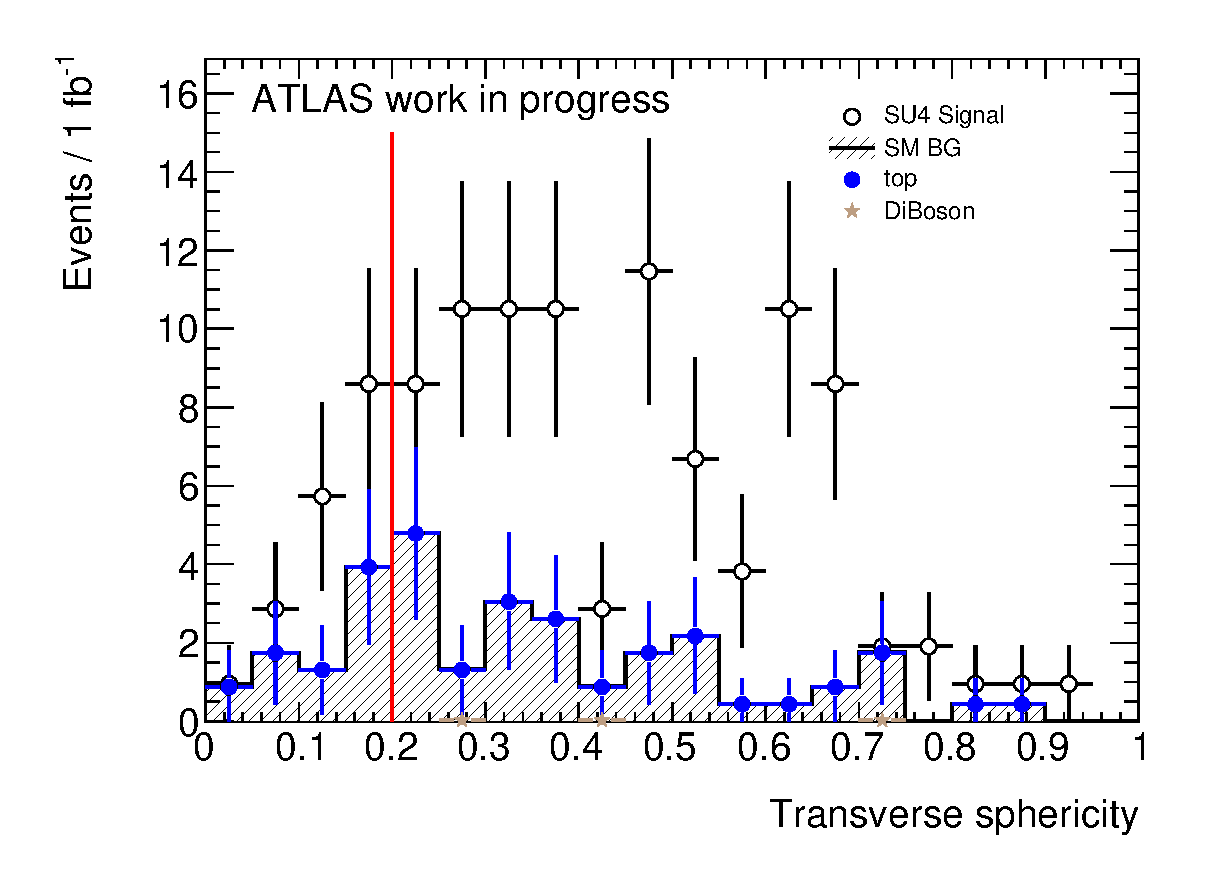
\includegraphics[width=.9\textwidth]{img/Canvas4j}
      \caption{Transverse sphericity distribution after 4 jet selection.}
      \label{fig:Canvas4j}
     \end{minipage}
    \end{figure}
   \begin{figure}\centering
    \begin{minipage}[c]{.3\textwidth}\centering\vfill
     \includegraphics[width=.95\textwidth]{img/susydoubledecay}
     \caption{A system of supersymmetric decays with 2 leptons and 2 jets in
     the final state.}
     \label{fig:susydoubledecay}
    \end{minipage}
    \begin{minipage}[c]{.3\textwidth}\centering\vfill
     \includegraphics[width=.95\textwidth]{img/2jttbardecay}
     \caption{A di-leptonic $t\bar{t}$ decay with 2 leptons and 2 jets in the
     final state.}
     \label{fig:2jttbardecay}
    \end{minipage}
    \begin{minipage}[c]{.3\textwidth}\centering\vfill
     \includegraphics[width=.95\textwidth]{img/4jttbardecay}
     \caption{A semi-leptonic $t\bar{t}$ decay with 1 lepton and 4 jets in the
     final state.}
     \label{fig:4jttbardecay}
    \end{minipage}
   \end{figure}
   \begin{block}{Control sample}
   The absolute number of events carries a large uncertainty due to our models
   of the processes. This section outlines how we can make these selections, but
   use data to provide background estimates resulting in lower
   uncertainties.
   
   The example Feynmann diagram in Fig.~\ref{fig:susydoubledecay} has a final
   state of 2 leptons, 2 light quarks and missing energy in the form of
   neutrinos and the lightest supersymmetric particle (LSP), in this model, the
   neutralino. For a selection optimised for events like these, we can estimate
   the top background by forming a control sample from a region where the
   background is strongly enhanced. For a search channel of $N$ jets and $M$
   leptons, we can look into a channel with $N+2$ jets and $M-1$ leptons. In top
   decay systems, this selects events where a W boson from a top decays
   leptonically in the search channel, and hadronically in a corresponding event
   in the control region.
   
   In the $N=2, M=2$ search channel, $t\bar{t}$ with a
   final state such as Fig.~\ref{fig:2jttbardecay} is the main background to the
   search. The control sample can be formed with a selection for events where
   $N=4, M=1$. This region would be composed mostly of events with the topology
   of Fig.~\ref{fig:4jttbardecay}.
   
   For the events in the control sample, we can simulate the kinematic variables
   for top events in the signal region by attempting to identify a pair of
   jets consistent with coming from a W. Replacing these with a simulated lepton
   and neutrino, we should reproduce a sample consistent with the background of
   the signal region.
% and then we put in two normal sized columns
   \end{block}
   \vskip2ex
%--Examples block---------------------------------------------------------------
   \begin{block}{Analysis strategy}
    After preparing a search and a control sample, we must relate the number of
    events in the control sample to the number expected under a background only
    hypothesis. A ratio can be formed between the samples as
    \begin{equation}
     \tau = \frac{n\left(t\bar{t}\text{ accepted
     in }N+2\text{ jet, }M-1\text{ lepton
     selection}\right)}{n\left(t\bar{t}\text{ accepted
     in }N\text{ jet, }M\text{ lepton selection}\right)}.
     \label{eq:ratio}
    \end{equation}
    Having estimated $\tau$ from data, the observation of experimental data can
    be modelled with Poisson statistics. The control region $m$ has expectation
    value,
    \begin{equation}
     E[m] = \tau b,
    \end{equation}
    where $b$ is the background to the search selection and $\tau$ is per
    Eq.\ref{eq:ratio}. Using this value of $b$, the signal expectation is;
    \begin{equation}
     E[n] = \mu s + b.
    \end{equation}
    Observing $\mu$ with a positive value indicates a discovery of beyond the
    standard model physics. Uncertainty from the absolute normalisation of the
    Monte Carlo is removed, only the relative uncertainty and the statistical
    error impact the measurement. It is expected that the normalisation of the
    Monte Carlo has a larger uncertainty than the ratio formed in
    Eq.\ref{eq:ratio} such that this analysis will achieve a higher
    significance, or make an earlier discovery.
   \end{block}
   \vskip2ex
  \vskip2ex
%--Examples block---------------------------------------------------------------
   \begin{block}{Multivariate techniques}
    In addition to improving the estimate of backgrounds to the search,
    the selection criteria can be optimised to increase signal to background
    ratios in the selections. Multivariate techniques combine variables from
    events and output one test statistic indicating to what degree the event
    appears like signal or background. This can create an selection criteria
    with greater significance than cuts on individual variables.
    
    By comparing the output distribution of a multivariate classifier under some
    top enhancement cuts and some Supersymmetry enhancing cuts, the model
    dependency the classifier may have formed in training on Monte Carlo events
    can be limited. The application of boosted decision trees for this role is
    under investigation to enhance this analysis.
   \end{block}
   \vskip2ex
%--Conclusion block-------------------------------------------------------------
   %\begin{alertblock}{Conclusion}
    %This analysis is under ongoing development but could form an early search
    %for supersymmetry. The impact of more backgrounds upon the samples
    %must be studied, along with how Supersymmetry may contaminate the
    %control sample. Research at royal holloway focuses on optimising selections
    %for high purity controls and using multivariate classifiers to reduce
    %reliance on Monte Carlo.
   %\end{alertblock}
%--References block-------------------------------------------------------------
   \begin{alertblock}{References}
    \begin{thebibliography}{7}
     \small %small is better for refs
       \bibitem{7tevNote} The ATLAS collaboration, \textit{Prospects for
       Supersymmetry discovery based on inclusive searches at a 7 TeV
       centre-of-mass energy with the ATLAS detector}, ATL-COM-PHYS-2010-336.
       \bibitem{CSCSUSY} The ATLAS collaboration, \textit{Expected Performance
       of the ATLAS Experiment}, CERN-OPEN-2008-020 (pg1514+).
    \end{thebibliography}
   \end{alertblock}
  \end{column}
 \end{columns}
\end{frame}
\end{document}
